\documentclass{beamer}

\usepackage[frenchb]{babel}
\usepackage[utf8]{inputenc}
\usepackage{default}
\usepackage{multimedia}

\usetheme{Luebeck}
%\setbeamercolor*{palette primary}{use=structure,fg=white,bg=gray}
%\setbeamercolor*{palette quaternary}{fg=white,bg=black}

\title[BMF 7robot 2013-2014]{BMF de 7Robot 2013-2014}
\author{7Robot}
\date{\today}

\setbeamertemplate{navigation symbols}{
  \insertframenavigationsymbol % Icône slide
  \insertbackfindforwardnavigationsymbol % Icône backfindforward
}
\setbeamertemplate{background canvas}{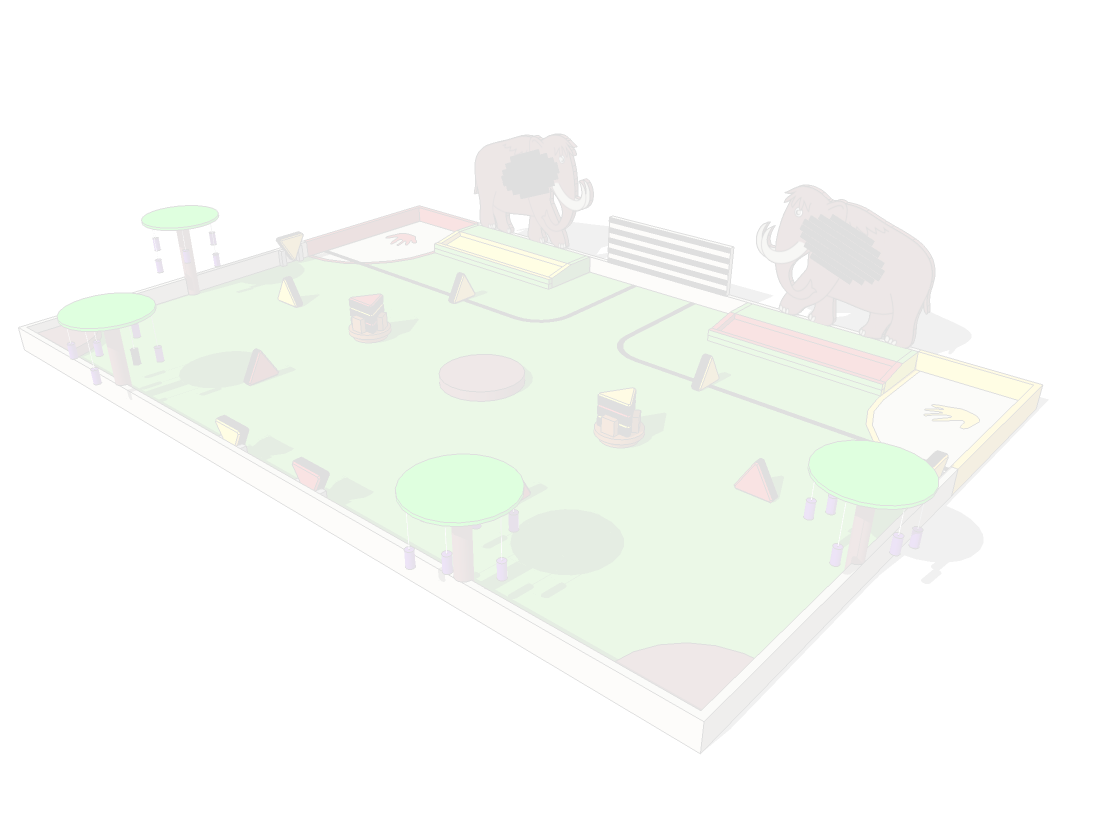
\includegraphics[width=\paperwidth,height=\paperheight]{../images/fond.png}}

\AtBeginSection[]{
  \begin{frame}
  \tableofcontents[currentsection, hideothersubsections]
  \end{frame} 
}

\begin{document}

\begin{frame}
  \titlepage
\end{frame}

\begin{frame}
  \tableofcontents
\end{frame}

\section{Les activités du club}
  \subsection{Coupe Freescale}
    \begin{frame}
Course de voitures miniatures automatiques.
Circuit constitué d'une ligne noire : faire un tour le plus vite possible.

Qualifications française organisée à l'N7 cette année.

\begin{block}{Résultats}
    2è, qualifiés pour la finale européenne en Allemagne.
\end{block}

\end{frame}

  \subsection{Coupe de France de Robotique}
    \begin{frame}
   \begin{center}
      
\includegraphics[width=0.6\textwidth]{../images/prehistobot.png}\\
      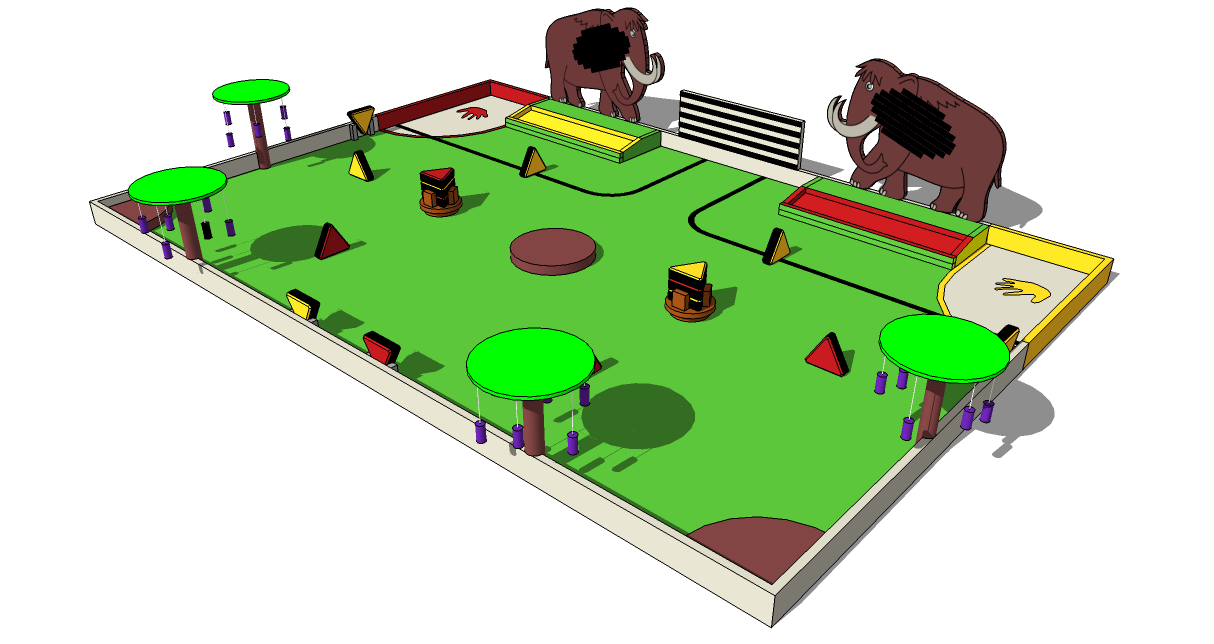
\includegraphics[width=\textwidth]{../images/table.png}
   \end{center}
\end{frame}

\begin{frame}
   La coupe de France de robotique est un événement annuel qui se passe à la Ferté Bernard.
   \begin{center}
      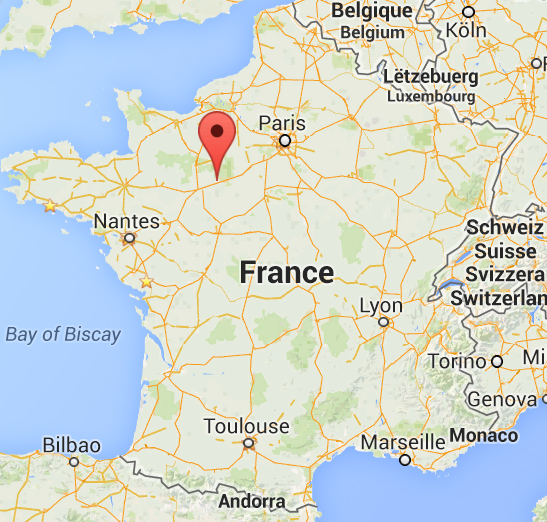
\includegraphics[width=0.4\textwidth]{../images/ferte.png}
   \end{center}
\end{frame}

\begin{frame}
   \begin{itemize}
      \item Près de 200 équipes (asso ou étudiante)
      \item Des étudiants ingénieurs de toute la France
      \item une compétition européenne (Eurobot)
   \end{itemize}
\end{frame}


\section{Bilan financier}
    \subsection{Recettes}
    \begin{frame}
   \begin{itemize}
      \item Subventions AEn7 : 2 900 €
      \item Elsys design : 700 €
   \end{itemize}
\end{frame}

    \subsection{Dépenses faites}
    \begin{frame}
   \begin{itemize}
      \item Semaine de bar : 310,87 € de perdus
      \item Outillage : 257,92 €
      \item Intelligence : 170,68 €
      \item Électronique : 116,47 €
      \item Motorisation : 263,95 €
      \item Capteurs : 106,50 €
      \item Mécanique : 124,64 €
      \item Divers : 133,22 €
   \end{itemize} 
Total : 1484,25 €
\end{frame}

    \subsection{Dépenses prévues}
    \begin{frame}
   Dépenses prévues :
   \begin{itemize}
       \item Voyage coupe de France : 600€
       \item Connectique : 20€
       \item Aspirateur : 50€
       \item Roues : 20€
       \item Batteries et chargeurs: 120€
       \item Dernière minute coupe de France : 200€
   \end{itemize}
   TOTAL : \textbf{1010€}
\end{frame}

    \subsection{Bilan}
    \begin{frame}
   \begin{itemize}
      \item Dépenses : 1484,25 €
      \item Dépenses prévues : 1010 €
      \item Recettes : 3 600 €
   \end{itemize}
   Bilan : \textbf{1105,75 €}
\end{frame}

  
\end{document}
